%
\section{Background}\label{sec:background}
%
\subsection{Open-source Software}
At a fundamental level, it's a software code that's available for all users to inspect, modify, copy and use in almost any way they choose. The first evolution of open-source software happened in the 1970's by Richard Stallman \cite{zh2011}. Commercial software often called proprietary software also has additional licensing that further prohibits people from attempting to reverse engineer or modify this process but in open-source software, the original source code is made available alongside the final executable program. This means any developers or programmers can modify the application to improve or customize it. The students also can study how the programs were written and the programs can be easily copied and distributed over the internet with the help of cloud repositories \cite{MiViIa2013}. Supporters of open-source believe open collaboration allows the software to evolve via the contribution of many users and also they believe people should have the right to use their software in whatever way they want without licensing restrictions. The term open-source has made many impacts in computer science practising whereas a lot of technologies have been built and distributed by a permissive license generally. The open-source software focuses more on the term “free” which helps to build open and transparent software systems. It also helps to improve the project becoming reliable and scalable so that it will help the digital economy to grow \cite{MiViIa2013}.
%
\subsection{National Vulnerability Database}
The \acs{NVD} is one of the largest and most effective databases which is used to report all known vulnerabilities for both commercial and open- source components. It was governed and operated under the US National Institute of Standards and Technology(NIST) from 2005. This organization is sponsored by the Department of Homeland Security's National Cybersecurity and Communications integration center and Network Security deployment[13]. The information which has been provided by the \acs{NVD} database helps the developer or security member to help track the software security. The information from \acs{NVD} helps to analyse the software security vulnerability of an \acs{OSS} component. It also helps the user to know what type of issues are in it and also helps the user to move further. A section of \acs{NVD} also provides information on \acs{CVE} as well as the information source, which is usually from the MITRE corporation \cite{TheNVD}. Figure~\ref{fig:vulgraph} will show us how far an \acs{OSS} component has impacted all these years. This information is gathered by \acs{NVD} with the help of the CVSS V2 and CVSS V3 data. The \acs{NVD} also gives us the history of all \acs{OSS} components with the help of MITRE’s \acs{CVE} dictionary[13]. The vulnerabilities of each component are discovered by the security researchers or organization and they will report this vulnerability to CVE. Once the rectified vulnerability is reported to the product owner or open-source project community to resolve it , the report will stay private for 60 to 90 days with \acs{CVE} before going public. The information from the \acs{NVD} is very useful to the consumers who use it so that they can protect themselves from the vulnerability but at the same time a hacker can also see the vulnerability of software before the consumer does. Once the threat of an \acs{OSS} component is received by the \acs{CVE} then this information is passed on to the \acs{NVD} database and will be available in search.

\begin{figure}[h!]
	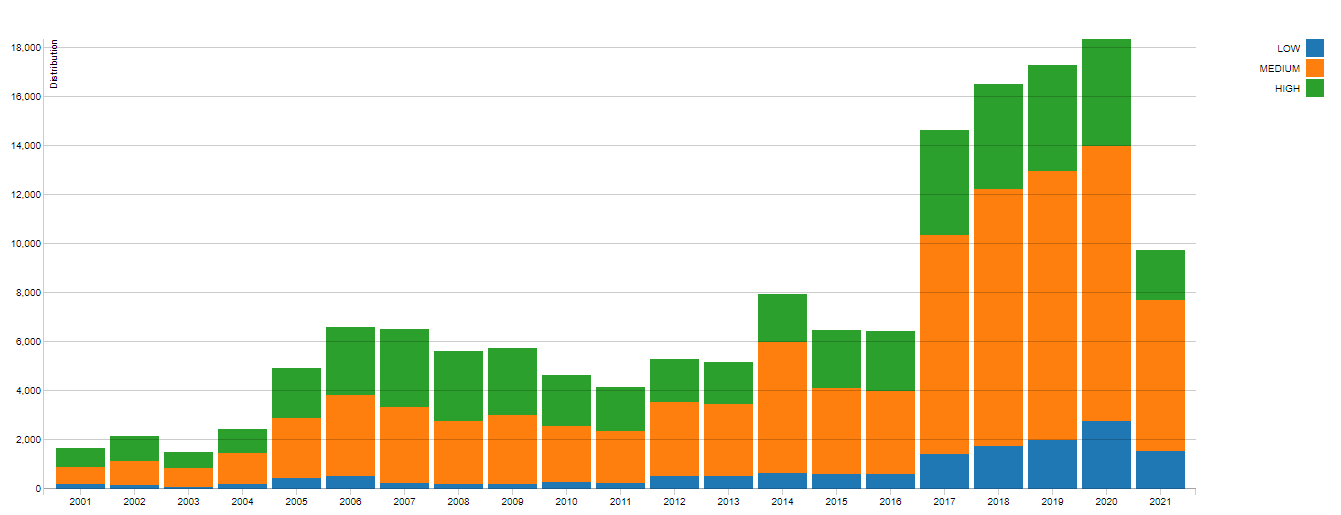
\includegraphics[width=15cm]{includes/vulgraph.PNG}
	\centering
	\caption{\acs{CVSS} Severity Distribution Over Time \cite{NVDgraph}}
	\label{fig:vulgraph}
\end{figure}
%
\subsection{Common Vulnerabilities \& Exposure}
The \acs{CVE} is built for one main purpose which is to identify, describe and catalog the cybersecurity vulnerabilities. Each Vulnerability will have one \acs{CVE} record in the catalog. All these vulnerabilities are discovered by the security expert  who works for an organization or independent which is partnered with \acs{CVE}. The \acs{CVE} program was found in 1999 first and it is runned by the Department of Homeland Security(DHS) and Cybersecurity and Infrastructure Security Agency(CISA). The \acs{CVE} and \acs{NVD} sound like they are the same but they are totally two different programs. Whereas the \acs{CVE} record contains the id number, description and a public reference of a known vulnerability, \acs{NVD} is a database which is used to list all the \acs{CVE} records of each vulnerability. The sponsors of the \acs{CVE} program decided to leave this information publicly accessible. The \acs{CVE} can also be used to integrate with security tools and services by an individual or organization. The users have all access to copy the record, reference the information or analyse the record without modifying it. The users can also link a \acs{CVE} record to another vulnerability under some terms and conditions. The \acs{CVE} provides a generic identifier for vulnerabilities  which helps the user to identify the information to access accurately and easily \cite{cve}. 
%

\subsection{Data Scraping}
Data exists everywhere in different formats like web pages to printed materials and as we established before there’s a lot of value that can be found in the right set of data. Data scraping is a process that extracts data from tables or other structured document formats and converts them into a format that can be easily processed or analyzed. It is useful because not all data sources provide ready-to-analyze, pre-formatted data. The data scraping plays a part in unlocking this value. Data scraping refers to the process of retrieving data from one format into a more useful format for further processing or analysing. In some scenarios the data might be extracted from similar data sets from two different sources. In that case the data has to be reviewed and processed to make sure they are both formatted equally. When it comes to different types of data sources there are endless ways in which data can be formatted. The two of the biggest categories of data sources are digital and physical sources \cite{NaJaMa2018}.
\paragraph{}
Data extraction can be categorized in two types: Logical and Physical extraction. Logical extraction will extract less information because it will consume less time and is a lot easier and it is categorized into two types: which is Full and Incremental extraction. Physical extraction is the opposite of logical extraction where it consumes more time but the outcome of this extraction will give you more information. Physical extraction is categorized in two types: Online and Offline extraction \cite{DataWH}.
%
\subsection{Vulnerability Analysis}
As businesses today increase their dependence on information technology including the cloud, IoT devices, mobile and social, their cyber risk continues to rise. However, a vulnerability management program can help to identify the weakness before it creates any major issues. Stats say 95\% of all cyber attacks exploit known vulnerabilities and on an average of 15,000 new vulnerabilities are discovered each year. So constant vigilance is required to evaluate IT security posture, discover weaknesses and respond appropriately. The key to responding to this more dangerous threat environment is a robust vulnerability analysis program. A Formal process that identifies and quantifies the security weakness including your application software, hardware and network. A vulnerability analysis should give a clean and clear report of what your environment needs attention and where on the list of priorities it lies. Identifying vulnerabilities is important  because unlike the targeted attacks which dominated the landscape previously. Today’s advanced attacks are programmed to search for vulnerabilities in a system and automatically start their attack process. Therefore it is critical to defend even if your organization is not a high priority target.The vulnerabilities can be scored based on the risk, impact and potential exploitation of the weakness.
\paragraph{}
The vulnerability analysis for open-source software should be imposed because software selection is essential in terms of information security. The quality of software selection should be strong so that we can reduce the risk of information security \cite{KeJaSa2005}. Vulnerability is also known as vulnerability assessment, “it is a mechanism that defines, identifies and classifies the security holes” \cite{KeJaSa2005}. The vulnerability assessment will also provide deep insight, knowledge and threats about the software to an organization or individual. There are several types of vulnerability analysis: Network-based analysis, Host-based analysis, Wireless network analysis, Application analysis and Database analysis.
\subsection{Dependency Manager}
A good design of software design concerns the software to be built from smaller, single-purpose modules with well defined interfaces and top of that keeping with the concept of software reuse. As a result of the broad adoption of open-source software, most of the softwares built now is dependent on softwares which is built by others. So to monitor all these dependencies used inside a software requires a dependency manager. A dependency is an external software module where it can contain one single file or a group of files clubbed together and can be used for performing specific tasks. Software modules known as dependency managers coordinate the integration of external libraries or packages into bigger applications. All dependency managers use a specific configuration file which consists of: dependency name, dependency version and repository of the dependency.The most common dependency manager’s configuration files are composer.json, package.json, build.gradle and pom.xml. All the initialised dependencies of the project are fetched from the repository by using their name and version. In some cases there are few dependency managers that have their own repository like maven central for maven and gradle projects, npm for npm based projects and packagist for composer projects \cite{Ma2017}. The dependency manager is required for two main reasons which is: i,to give a confirmation that both the development and production environment uses the same dependency and its version. ii, to keep the dependency up to date \cite{Dm2018}.
%
\subsubsection{Components of Dependency Manager}
The following are typical components of a dependency management system \cite{DataWH}:
\begin{description}
	\item [$\bullet$ Module:] This component can be used in all sorts of projects and these can be called packages or libraries based on the programming language. The modules come with the information of what dependencies are required for a specific module.
	
	\item [$\bullet$ Manifest file:] This file records all the dependencies of the project. It contains all the meta information of the project. 
	
	\item [$\bullet$ Lock file:] This file usually captures all the meta information of the dependencies and converts into a dependency source tree and also makes the versions immutable.
	
	\item [$\bullet$ Repository:] In most cases each dependency has its own repository where the dependencies will be fetched directly from the repository to the project. For example, maven and gradle project dependencies are fetched fromMaven Central.
	
	\item [$\bullet$ Dependency Constraint:] There will be a dependency constraint in the manifest file where it allows only the required version of the project.
	
	\item [$\bullet$ Resolution Rule:] This is a rule where every dependency manager has to select the correct dependency version to the project.
	
\end{description}

%
